% "{'classe':('PSI','PT'),'chapitre':'slci_rp','type':('colle'),'titre':'Quille pendulaire', 'source':'Concours Commun Mines Ponts 2014','comp':('C1-02','C2-04'),'corrige':True}"
%\setchapterimage{bandeau}
\chapter*{Colle \arabic{cptColle} \\ 
Quille pendulaire \ifnormal $\star$ \else \fi \iftdifficile $\star\star\star$ \else \fi  -- 
\ifprof Corrigé \else Sujet \fi}
\addcontentsline{toc}{section}{Colle \arabic{cptColle} :
Quille pendulaire \ifnormal $\star$ \else \fi \iftdifficile $\star\star\star$ \else \fi  -- 
\ifprof Corrigé \else Sujet \fi}

\iflivret \stepcounter{cptColle} \else
\ifprof  \stepcounter{cptColle} \else \fi
\fi

\setcounter{question}{0}
\marginnote{Concours Commun Mines Ponts 2014.}
\marginnote[1cm]{
\UPSTIcompetence[2]{C1-02}
\UPSTIcompetence[2]{C2-04}}

\begin{marginfigure} [4cm]
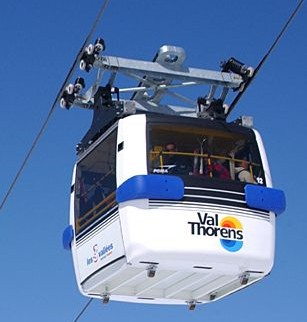
\includegraphics[width=\linewidth]{fig_00}
\end{marginfigure}


\section*{Mise en situation}
\ifprof
\else

Les actions de l'air et de l'eau permettent au voilier d'avancer mais provoquent aussi son inclinaison autour de l'axe longitudinal $\vect{z_N}$. C’est le phénomène de gîte. Pour contrebalancer ce mouvement et éviter que le voilier ne se couche sur l’eau, la quille joue le rôle de contrepoids. 


%\begin{center}
%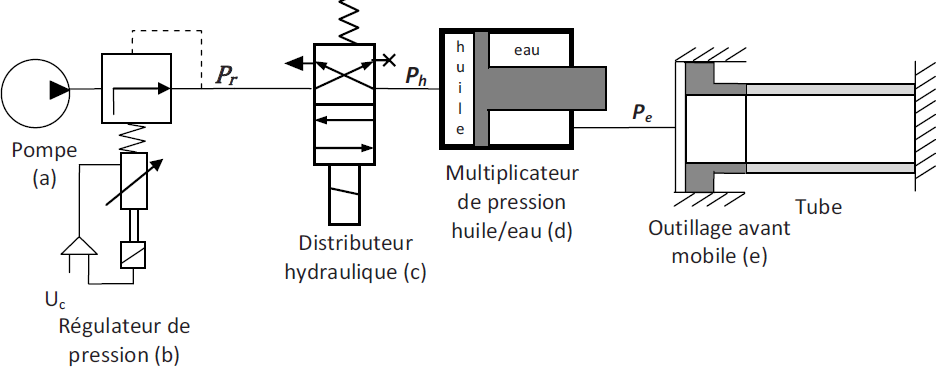
\includegraphics[width=.8\linewidth]{fig_01}
%%\textit{}
%\end{center}

Une évolution récente des voiliers de course océanique a été de les doter d’une quille pendulaire. Cette quille est en liaison pivot d’axe $\left(O,\vect{z}_N \right)$ avec la coque du navire et peut être orientée d’un côté ou de l’autre du navire. Une fois l’orientation désirée obtenue, tout mouvement dans la liaison pivot est supprimé par le blocage en rotation de celle-ci. 

\begin{marginfigure}[-2cm]
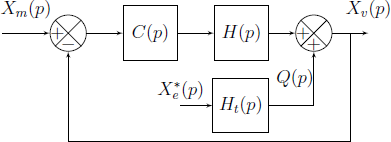
\includegraphics[width=\linewidth]{fig_03}

\caption{Modèle volumique 3D}
\end{marginfigure}


Afin de garantir sa répétabilité, la mise en position angulaire de la quille fait l’objet d’un contrôle par une boucle d’asservissement, dont le cahier des charges est donné en fin de sujet.
%
%\begin{center}
%\begin{tabular}{|p{.7\linewidth}|c|}
%\hline
%Exigences & Niveau \\
%\hline\hline
%Stabilité : & \\
%C11 : Marge de gain & \SI{10}{dB} \\
%C12 : Dépassement vis-à-vis d'une entrée en échelon & Aucun \\
%\hline
%Rapidité :  & \\
%C21 : Temps de réponse à 5\, \% & \SI{4}{s} maxi  \\
%C22 : Vitesse angulaire de rotation de la quille & $8\degres/\text{s}$  maxi\\
%\hline
%Précision & \\
% C3 : Erreur statique vis-à-vis d'une entrée en échelon & Nulle \\
%\hline
%\end{tabular}
%\end{center}
\fi


\begin{obj}
L'objectif de proposer un correcteur permettant de vérifier l'ensemble des critères du cahier des charges. 

\end{obj}
\subsection*{Modélisation du vérin}

\ifprof
\else
La quille est manoeuvrée par deux vérins hydrauliques. Chacun d’eux est piloté par une servovalve de débit. Ce composant délivre un débit $q(t)$ proportionnel à sa tension de commande $v(t)$. Lors d’une manoeuvre de quille un seul de ces vérins est moteur et alimenté en pression via sa servovalve. L’autre est laissé dans une configuration où sa tige est libre de tout mouvement. Le déplacement terminé, la quille est verrouillée en position par un système de blocage non étudié dans ce sujet qui interdit toute circulation de fluide entre vérins et servovalves. L’angle de rotation de la quille par rapport au bâti est mesuré par un capteur potentiométrique.


Lors d’un déplacement de la quille, les mouvements d’oscillation du cylindre de vérin par rapport à la coque étant de faible amplitude et s’effectuant à de faibles vitesses, on se place dans une situation où le corps de vérin est considéré comme fixe. La tige est alors considérée en mouvement de translation galiléen.
On considère également que les mouvements étudiés sont de petits mouvements autour d’une position moyenne et que l’hypothèse des conditions initiales nulles est valide. Dans ces conditions, le comportement du vérin est défini par le modèle continu ci-dessous.


\footnotesize
\begin{center}
\begin{tikzpicture}
\sbEntree{E}

\sbBloc[3]{b0}{$A_1$}{E}
    \sbRelier[$Q(p)$]{E}{b0}


\sbComp{c1}{b0}
    \sbRelier{b0}{c1}

\sbBloc[1]{b1}{$A_2$}{c1}
    \sbRelier{c1}{b1}
    
\sbBloc[3]{b11}{$A_3$}{b1}
    \sbRelier[$\Sigma(p)$]{b1}{b11}


\sbComph{c2}{b11}
    \sbRelier{b11}{c2}

\sbBloc{b2}{$A_4$}{c2}
    \sbRelier{c2}{b2}
    

\sbSortie[4]{S}{b2}
    \sbRelier{b2}{S}
    \sbNomLien[0.8]{S}{$X(p)$}
  
\sbRenvoi{b2-S}{c1}{}

\draw [latex-] (c2) --++ (0,1) node[left] {$F_R(p)$};

\end{tikzpicture}
\end{center}
\normalsize

On a : 
\begin{itemize}
\item $q(t)=S\dfrac{\dd x(t)}{ \dd t}+\dfrac{V}{2B}\dfrac{\dd \sigma(t)}{\dd t}$ (a);
\item $M\dfrac{\dd^2 x(t)}{\dd t^2} = S \sigma(t) - kx(t)-\lambda \dfrac{\dd x(t)}{\dd t} - f_R(t)$ (b).
\end{itemize}

On a :
\begin{itemize}
\item $\mathcal{L}\left(q(t)\right)=Q(p)$ : débit d’alimentation du vérin $\left[\text{m}^3\text{s}^{-1}\right]$;
\item $\mathcal{L}\left(\sigma(t)\right)=\Sigma(p)$ : différence de pression entre les deux chambres du vérin $\left[\text{Pa}\right]$;
\item $\mathcal{L}\left(x(t)\right)=X(p)$ : position de la tige du vérin $\left[\text{m}\right]$;
\item $\mathcal{L}\left(f_R(t)\right)=F_R(p)$ : composante selon l'axe de la tige du vérin de la résultante du torseur d'inter-effort de la liaison pivot entre tige et quille $\left[\text{N}\right]$.
\end{itemize}
Les constantes sont les suivantes :
\begin{itemize}
\item $S$ : section du vérin $\left[\text{m}^2\right]$;
\item $k$ : raideur mécanique du vérin $\left[\text{N\,m}^{-1}\right]$;
\item $V$ : volume d'huile de référence $\left[\text{m}^{3}\right]$;
\item $B$ : coefficient de compressibilité de l'huile $\left[\text{N\, m}^{-2}\right]$;
\item $M$ : masse équivalente à l'ensemble des éléments mobiles ramenés sur la tige du vérin $\left[\text{kg}\right]$;
\item $\lambda$ : coefficient de frottement visqueux$\left[\text{N\,m}^{-1}\text{s}\right]$.
\end{itemize} 

\fi
\question{Donner les expressions des fonctions de transfert $A_1$, $A_2$, $A_3$ et $A_4$ en fonction de la variable
complexe $p$ et des constantes.}
\ifprof
\begin{corrige}
D'une part, on transforme les équations dans le domaine de Laplace : 
$Q(p)=S p X(p)+\dfrac{V}{2B} p \Sigma(p)$ et
$Mp^2 X(p) = S \Sigma(p) - kX(p)-\lambda p X(p) - F_R(p)$.

En utilisant le schéma-blocs, on a $\Sigma(p)=A_2\left(A_1Q(p)-X(p)\right) = A_1A_2Q(p)-A_2X(p)$.

Par ailleurs $\Sigma(p)=\dfrac{Q(p)-S p X(p)}{\dfrac{V}{2B} p}= Q(p)\dfrac{2B}{Vp}-  X(p)  \dfrac{S2B}{V} $. On a donc $A_2 = \dfrac{S2B}{V} $, $A_1 A_2 = \dfrac{2B}{Vp}$ soit $A_1  = \dfrac{2B}{Vp}\dfrac{V}{S2B}= \dfrac{1}{Sp}$. 


On a aussi $X(p)=A_4\left(-F_R(p)+A_3\Sigma(p)\right) =-A_4F_R(p)+A_3A_4\Sigma(p)$. Par ailleurs,
$X(p) \left(Mp^2  +\lambda p  + k\right)= S \Sigma(p) - F_R(p) \Leftrightarrow X(p) =  \dfrac{S \Sigma(p)}{Mp^2  +\lambda p  + k}-\dfrac{F_R(p)}{Mp^2  +\lambda p  + k}$. On a donc : $A_4 = \dfrac{1}{Mp^2  +\lambda p  + k}$ et $A_3 = S$.

Au final,  $A_1=\dfrac{1}{Sp}$,  $A_2 = \dfrac{S2B}{V} $,  $A_3 = S$  et $A_4 = \dfrac{1}{Mp^2  +\lambda p  + k}$.
\end{corrige}
\else
\fi

\ifprof
\else

Le schéma-blocs de la figure précédente peut se mettre sous la forme suivante. 

\begin{marginfigure}
\footnotesize
\begin{center}
\begin{tikzpicture}
\sbEntree{E}

\sbBloc[3]{b1}{$H_1$}{E}
    \sbRelier[$Q(p)$]{E}{b1}


\sbComph{c1}{b1}
    \sbRelier{b1}{c1}
  
\sbBloc{b2}{$H_2$}{c1}
    \sbRelier{c1}{b2}

\sbSortie{S}{b2}
    \sbRelier{b2}{S}
    \sbNomLien[0.8]{S}{$X(p)$}

%\sbBloc[3]{b11}{$A_3$}{b1}
%    \sbRelier[$\Sigma(p)$]{b1}{b11}
%
%
%\sbSumh{c2}{b11}
%    \sbRelier{b11}{c2}
%
%\sbBloc{b2}{$A_4$}{c2}
%    \sbRelier{c2}{b2}
%    
%
%\sbSortie[4]{S}{b2}
%    \sbRelier{b2}{S}
%    \sbNomLien[0.8]{S}{$X(p)$}
%  
%\sbRenvoi{b2-S}{c1}{}
%
\draw [latex-] (c1) --++ (0,1) node[left] {$F_R(p)$};

\end{tikzpicture}
\end{center}
\normalsize
\end{marginfigure}
\fi

\question{Donner les expressions des fonctions de transfert $H_1$
et $H_2$ en fonction de $A_1$, $A_2$, $A_3$ et $A_4$, puis de la variable $p$ et
des constantes.}
\ifprof
\begin{corrige}
\textbf{Méthode 1 : Utilisation des relations précédentes}
On a $X(p)=\left(H_1Q(p)-F_R(p)\right)H_2(p)$. 

Par ailleurs, on a vu que $X(p)=A_4\left(-F_R(p)+A_3\Sigma(p)\right) $ et $\Sigma(p)=A_2\left(A_1Q(p)-X(p)\right)$. 

On a donc $X(p)=A_4\left(-F_R(p)+A_3  A_2\left(A_1Q(p)-X(p)\right)\right) $ $ \Leftrightarrow X(p)\left(1+A_2A_3A_4 \right)=A_4\left(-F_R(p)+A_3  A_2A_1Q(p)\right) $. On a donc 
$H_1(p)=A_1  A_2A_3$ et $H_2 = \dfrac{A_4}{1+ A_2A_3A_4 }$.

\textbf{Méthode 2 : Lecture directe du schéma-blocs}
Revient à utiliser la méthode précédente. 

\textbf{Méthode 3 : Algèbre de schéma-blocs}
Le schéma-blocs proposé est équivalent au schéma suivant. 

\footnotesize
\begin{center}
\begin{tikzpicture}
\sbEntree{E}

\sbBloc[3]{b0}{$A_1 A_2 A_3$}{E}
    \sbRelier[$Q(p)$]{E}{b0}

\sbComph{c2}{b0}
    \sbRelier{b0}{c2}
    
\sbComp{c1}{c2}
    \sbRelier{c2}{c1}

\sbBloc{b1}{$A_4$}{c1}
    \sbRelier{c1}{b1}
    

\sbSortie[4]{S}{b1}
    \sbRelier{b1}{S}
    \sbNomLien[0.8]{S}{$X(p)$}
      
      
\sbDecaleNoeudy[4]{S}{U}
\sbDecaleNoeudx[-2]{U}{U2}
\sbBlocr{r1}{$A_2 A_3$}{U2}


\sbRelieryx{b1-S}{r1}
\sbRelierxy{r1}{c1}


%    
%\sbBloc[3]{b11}{$A_3$}{b1}
%    \sbRelier[$\Sigma(p)$]{b1}{b11}
%
%
%\sbComph{c2}{b11}
%    \sbRelier{b11}{c2}
%
%\sbBloc{b2}{$A_4$}{c2}
%    \sbRelier{c2}{b2}
%    
%
%\sbRenvoi{b2-S}{c1}{}

\draw [latex-] (c2) --++ (0,1) node[left] {$F_R(p)$};

\end{tikzpicture}
\end{center}
\normalsize

On retrouve le même résultat que précédemment. 


$A_1=\dfrac{1}{Sp}$,  $A_2 = \dfrac{S2B}{V} $,  $A_3 = S$  et $A_4 = \dfrac{1}{Mp^2  +\lambda p  + k}$.


En faisant le calcul on obtient : 
$H_1(p)=\dfrac{2BS}{pV}  $ et $H_2 = \dfrac{\dfrac{1}{Mp^2  +\lambda p  + k}}{1+ \dfrac{2BS^2}{V}\dfrac{1}{Mp^2  +\lambda p  + k} }$  $= \dfrac{1}{Mp^2  +\lambda p  + k+ \dfrac{2BS^2}{V} }$.

\end{corrige}
\else
\fi

\question{Pour ce vérin non perturbé ($F_R=0$), donner sa fonction de transfert $X(p)/Q(p)$ en fonction de la variable $p$ et des constantes.}
\ifprof
\begin{corrige}
Dans ce cas, $\dfrac{X(p)}{Q(p)}=H_1(p)H_2(p)\dfrac{2BS}{p\left(MVp^2  +\lambda pV  + kV+ 2BS^2\right) }$.
\end{corrige}
\else
\fi

\ifprof
\else
Le schéma d’asservissement de la position angulaire de la quille représenté figure ci-dessous sera utilisé
pour la suite des questions. La perturbation représentée par $F_R(p)$ ne sera pas prise en compte.

\footnotesize
\begin{center}
\begin{tikzpicture}[scale=0.75, every node/.style={transform shape}]
\sbEntree{E}

\sbBloc[3]{b0}{$K'_C$}{E}
    \sbRelier[$\Theta_c(p)$]{E}{b0}


\sbComp[5]{c1}{b0}
    \sbRelier[$V_c(p)$]{b0}{c1}

\sbBloc[1]{b1}{$C(p)$}{c1}
    \sbRelier{c1}{b1}
    
\sbBloc[2.5]{b2}{$H_{\text{SV}}$}{b1}
    \sbRelier[$V(p)$]{b1}{b2}

\sbBloc[2.5]{b3}{$H_{1}$}{b2}
    \sbRelier[$Q(p)$]{b2}{b3}
    
\sbComph[3.5]{c2}{b3}
    \sbRelier{b3}{c2}

\sbBloc[1]{b4}{$H_2$}{c2}
    \sbRelier{c2}{b4}
    
\sbBloc[2.5]{b5}{$H_{\text{CIN}}$}{b4}
    \sbRelier[$X(p)$]{b4}{b5}

\sbSortie[2]{S}{b5}
    \sbRelier{b5}{S}
    \sbNomLien[0.8]{S}{$\Theta(p)$}
  

\sbDecaleNoeudy[4]{b3}{U}
\sbBlocr{r1}{$K_C$}{U}

\sbRelieryx{b5-S}{r1}
\sbRelierxy[$V_m(p)$]{r1}{c1}

%\sbRenvoi{b2-S}{c1}{}

\draw [latex-] (c2) --++ (0,1) node[left] {$F_R(p)$};

\end{tikzpicture}
\end{center}

\normalsize


On a :
\begin{itemize}
\item $\mathcal{L}\left(\theta_c(t)\right)=\Theta_c(p)$ : consigne de position angulaire $\left[\degres\right]$;
\item $\mathcal{L}\left(\theta(t)\right)=\Theta(p)$ : position angulaire de la quille $\left[\degres\right]$;
\item $\mathcal{L}\left(v(t)\right)=V(p)$ : tension de commande de la servo valve $\left[\text{V}\right]$;
\item $\mathcal{L}\left(v_c(t)\right)=V_c(p)$ : tension image de la consigne $\left[\text{V}\right]$;
\item $\mathcal{L}\left(v_m(t)\right)=V_m(p)$ : tension image de la position $\left[\text{V}\right]$.
\end{itemize}

On a de plus :
\begin{itemize}
\item $K_c$ : gain du capteur angulaire potentiométrique $\left[\text{V}/\degres\right]$;
\item $K'_c$ : gain du bloc d'adaptation réglé tel que $K'_c=K_c=\SI{1,1}{V/\degres}$;
\item $C(p)$ : correcteur de position;
\item $H_{\text{CIN}}$ : fonction de transfert de la chaîne de transformation de mouvement dont la loi
d’entrée/sortie est supposée linéaire dans le domaine d’utilisation. $H_{\text{CIN}}=K_{\theta}$ $\left[\degres.\text{m}^{-1}\right]$;
\item $H_{\text{SV}}$ : fonction de transfert de la servo valve.
\end{itemize}

\fi

%\subsection*{Modélisation de la servo valve : comportement pour une commande de grande amplitude}
%
%\ifprof
%\else
%La servovalve présente un fonctionnement non-linéaire provenant
%d’un phénomène de saturation qui est défini par la courbe de la
%figure suivante donnant les évolutions du débit $q(t)$ fourni par la
%servovalve en fonction de sa tension de commande $v(t)$.
%\begin{center}
%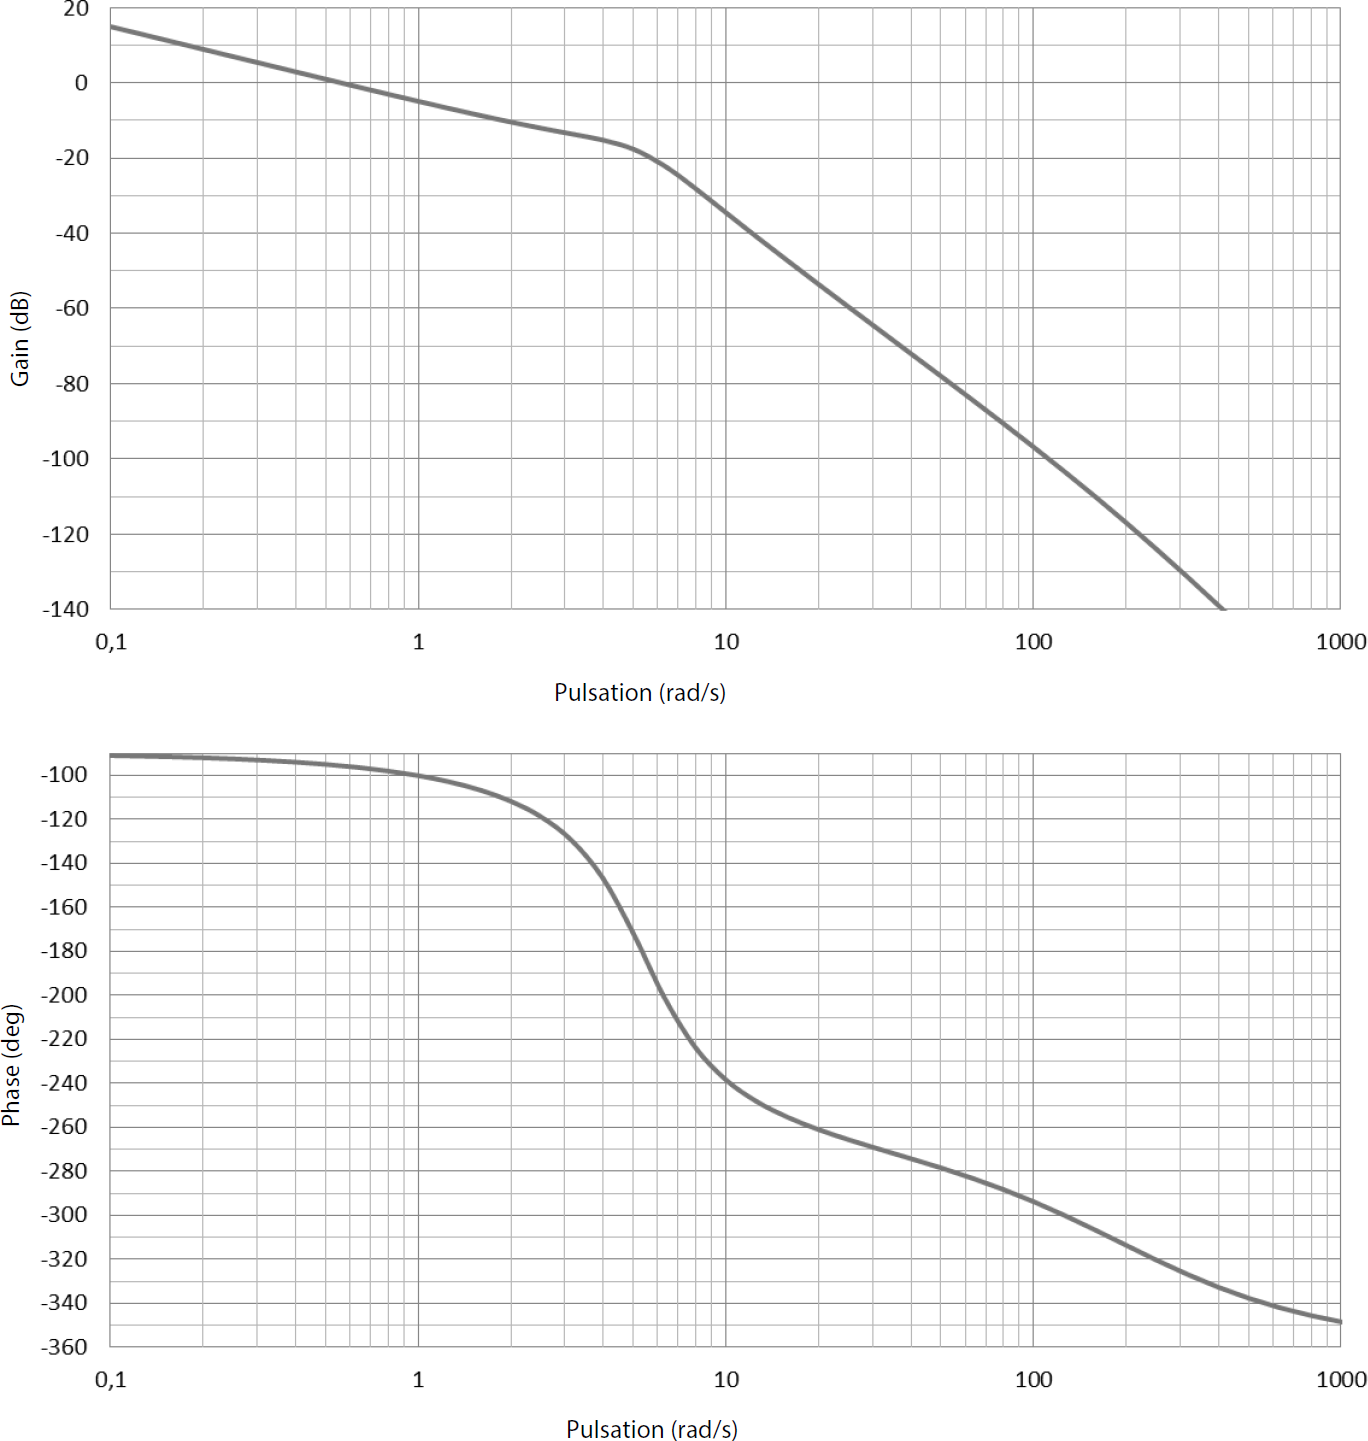
\includegraphics[width=.5\linewidth]{fig_04}
%
%\end{center}
%
%Ainsi :
%\begin{itemize}
%\item pour $v(t) > -v_{\text{max}}$ et $v(t) < v_{\text{max}}$ : $H_{\text{sv}} = K_{\text{sv}}$ $\left[\text{m}^3 \text{s}^{-1}\text{V}^{-1}\right]$
%\item pour $v(t) < -v_{\text{max}}$: $q(t) = -q_{\text{max}}$;
%\item pour $v(t) > v_{\text{max}}$ : $q(t) = +q_{\text{max}}$ , $v_{\text{max}} = \SI{10}{V}$.
%\end{itemize}
%Le système n’est pas encore corrigé, $C(p) =1$ et on souhaite simuler
%le fonctionnement où le navigateur veut déplacer la quille avec une
%consigne angulaire de position de 45\degres. Cette demande est modélisée
%par une consigne $\theta_c(t)$ en échelon, soit : $\theta_c(t)=\theta_0\,u(t)$ avec $\theta_0=45\degres$ et
%$u(t) = 0$ pour $t < 0$ et $u(t) = 1$ pour $t > 0$. La figure suivante présente dans ces conditions les évolutions temporelles de deux grandeurs de la boucle d’asservissement, le débit sortant de la servo valve
%$q(t)$ et la position angulaire de la quille $\theta(t)$.
%
%\begin{center}
%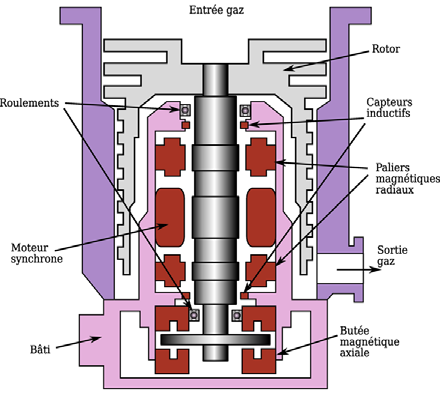
\includegraphics[width=\linewidth]{fig_05}
%\end{center}
%
%Sur la figure précédente, la courbe représentative de $q(t)$ présente un palier où $q(t)$ garde une valeur constante.
%\fi
%
%\question{À l’aide de la caractéristique de la servovalve :}
%\textit{
%\begin{enumerate}
%\item justifier ce palier et donner la valeur numérique de $K_{\text{SV}}$;
%\item indiquer sur la figure l’intervalle de temps où le retour d’information a une influence sur la
%commande du vérin et celui où il n’en a pas. Associer à chacun de ces intervalles le modèle utile :
%modèle en « boucle fermée » ou en « boucle ouverte ».
%\end{enumerate}}
%\ifprof
%\begin{corrige}
%En début de simulation, il y a une saturation du débit à \SI{20e-3}{m^3 s^{-1}}. La tension de commande en régime saturé étant de \SI{10}{V}, on a $K_{\text{SV}} = \SI{2e-3}{m^3 s^{-1}V^{-1}}$.
%
%Jusqu'à 1,9 seconde, le retour n'a aucune influence sur la commande. On est donc en BO. Au delà, la régulation entre en en jeu. On est donc en BF. 
%
%\end{corrige}
%\else
%\fi
%
%\question{Montrer, en précisant la ou les exigences mises en défaut, que le cahier des charges n’est pas respecté au niveau des critères « vérifiables ».}
%\ifprof
%\begin{corrige} ~\\
%
%\begin{center}
%\begin{tabular}{|l|c|l|l|}
%\hline
%Exigences & Niveau & Simulation & Validation  \\
%\hline\hline
%Stabilité : & & & \\
%C11 : Marge de gain & \SI{10}{dB} & -- & -- \\
%C12 : Dépassement vis-à-vis d'une entrée en échelon & Aucun & Dépassement faible& NON \\
%\hline
%Rapidité :  & &&\\
%C21 : Temps de réponse à 5\, \% & \SI{4}{s} maxi  & $\simeq \SI{2,5}{s}$& OUI\\
%C22 : Vitesse angulaire de rotation de la quille & $8\degres/\text{s}$  maxi & $\simeq \SI{20}{\degres.s^{-1}}$&NON\\
%\hline
%Précision & &&\\
% C3 : Erreur statique vis-à-vis d'une entrée en échelon & Nulle &Difficile à mesurer & -- \\
%\hline
%\end{tabular}
%\end{center}
%
%
%\end{corrige}
%\else
%\fi

\subsection*{Comportement pour une commande de faible amplitude}
\ifprof
\else
On étudie la réponse du système non corrigé ($C(p) = 1$) à une entrée échelon de 5\degres\;d’amplitude avec $F_R = 0$.
Le modèle de travail qui a permis de tracer les courbes de la figure précédente est :
$H_{\text{BO}}(p)=K_{\text{SV}} H_1 H_2 K_{\theta} K_C$ et $H_{\text{BO}}(p)=\dfrac{2,2}{p\left(1+0,12p + 0,04 p ^2  \right)}$.
\fi

%\question{Pour l’entrée définie ci-dessus, déterminer la valeur de la tension $v(t)$ à l’instant initial $t=0^{+}$, $v(0^{+})$. Expliquer succinctement que tout au long de ce fonctionnement, la servovalve fonctionnera sans saturer.}
%\ifprof
%\begin{corrige} En BO, on va avoir $v(0^{+})=5\cdot K'_C =\SI{5,5}{V}$. 
%
%$v(0^{+})<\SI{10}{V}$. On est ici en BO. La tension ne peut donc pas dépasser la tension de saturation. 
%\end{corrige}
%\else
%\fi
%
%
%\question{De quelle hypothèse générale d’étude des systèmes asservis ce constat participe-t-il ?}
%\ifprof
%\begin{corrige}
%Pour de telles tension, on est donc en régime \textbf{linéaire}.
%\end{corrige}
%\else
%\fi

\ifprof
\else
Une simulation de la réponse indicielle à cet échelon de 5\degres d’amplitude a permis de tracer les courbes de la
figure suivante, obtenues pour deux valeurs du correcteur proportionnel :
\begin{itemize}
\item $C(p) = 1$ : la courbe présente des dépassements, l'exigence 2.1.2 n'est pas validée;%le critère C12 n’est pas validé;
\item $C(p) = 0,44$ : toutes les exigences du domaine temporel sont vérifiées (2.1.2, 2.2.1; 2.2.2, 2.3.1).%(C12, C21, C22, C3).
\end{itemize}

\begin{marginfigure}
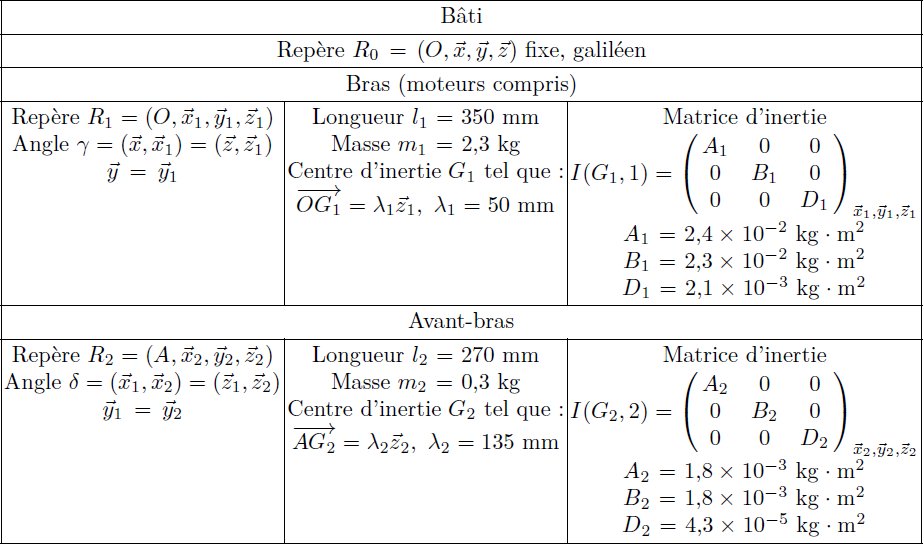
\includegraphics[width=\linewidth]{fig_06}
\end{marginfigure}

À l’utilisation, le correcteur proportionnel réglé à 0,44 n’a pas donné satisfaction car le mouvement saccadé
de la quille dû aux fluctuations de sa vitesse de rotation générait dans certaines conditions de navigation des
perturbations compromettant la stabilité de route du navire. L’examen attentif de cette réponse indicielle
fait apparaître la persistance d’un phénomène oscillatoire dont l’origine supposée se trouve dans le
caractère résonant du vérin.

\fi

\question{Tracer sur les figures suivantes les diagrammes d’amplitude asymptotiques de
Bode de $H_{\text{BO}}(p)$ en indiquant les valeurs numériques associées aux
points particuliers et la valeur des pentes.}
\ifprof
\begin{corrige}
On a : $H_{\text{BO}}(p)=\dfrac{2,2}{p\left(1+0,12p + 0,04 p ^2  \right)}$. En conséquences, $\dfrac{1}{\omega_0^2}={0,04}$ et $\omega_0 = \SI{5}{rad.s^{-1}}$ et $\dfrac{2\xi}{\omega_0}=0,12 \Leftrightarrow \xi=0,3$.


On a donc une asymptote de $-\SI{20}{dB/decade}$ pour $\omega<\SI{5}{rad.s^{-1}}$ et $-\SI{60}{dB/decade}$ pour $\omega>\SI{5}{rad.s^{-1}}$.

De plus, pour $\omega=\SI{5}{rad.s^{-1}}$, on a $20\log\dfrac{2,2}{5}=\SI{-7,1}{dB}$. 

\end{corrige}
\else
\fi

\ifprof
\else
\begin{center}
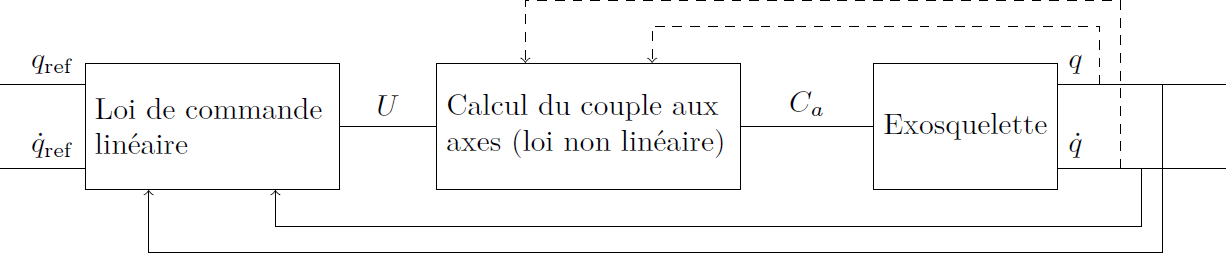
\includegraphics[width=\linewidth]{fig_07}
%\textit{}
\end{center}
\fi

\question{Déterminer par calcul la pulsation de résonance $\omega_r$ de cette fonction
de transfert.}
\ifprof
\begin{corrige}
On a $\omega_r = \omega_0\sqrt{1-2\xi^2}=5\times \sqrt{1-2\times 0,3^2}\simeq \SI{4,5}{rad.s^{-1}}$.
\end{corrige}
\else
\fi


\question{Évaluer littéralement puis numériquement à cette pulsation
$\omega_r$ la différence, notée $\Delta K$ et exprimée en dB, entre l’amplitude
de résonance et l’amplitude évaluée par le diagramme asymptotique.}
\ifprof
\begin{corrige}
L'amplitude de résonance ne dépend que du système du second ordre. On a alors (résultat de cours sur le second ordre) : 
$\Delta K = 20\log \left( \dfrac{1}{2\xi \sqrt{1-\xi^2}}\right)=20\log \left( \dfrac{1}{2\times 0,3 \sqrt{1-0,3^2}}\right)=\SI{4,8}{dB}$. 
\end{corrige}
\else
\fi

\ifprof
\else
\begin{marginfigure}
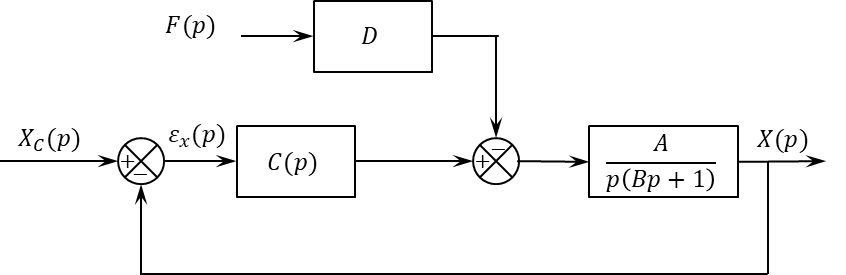
\includegraphics[width=\linewidth]{fig_08}
%\textit{}
\end{marginfigure}
\fi

 \ifprof
 \else
Pour éliminer le phénomène de résonance, on recherche l’expression de $C(p)$ permettant d’abaisser
l’amplitude de $\Delta K$ à la pulsation $\omega_r$. Le concepteur a choisi un correcteur à retard de phase de fonction de
transfert $C(p)=K_{\text{COR}} \dfrac{1+Tp}{1+bTp}$ avec $b>1$. Ce correcteur présente un extremum de la courbe de phase à la pulsation $\omega^{*}$ tel que : $\sin\left[\phi\left(\omega^{*}\right)\right]=\dfrac{1-b}{1+b}$ et $\omega^{*}=\dfrac{1}{T\sqrt{b}}$.


L’étude consiste à déterminer les valeurs de $T$ et $b$.

\fi

\question{Tracer sur la figure précédente, l'allure des diagrammes d’amplitude et de phase (asymptotiques et allure
de la courbe réelle) de Bode de ce correcteur pour $K_{\text{COR}} =1$. Préciser les expressions littérales des
pulsations caractéristiques.}
\ifprof
\begin{corrige}
On a  $b>1$ donc $T<bT$ et $\dfrac{1}{T}>\dfrac{1}{bT}$. 

Pour $\omega<\dfrac{1}{bT}$ on a donc un gain de pente nulle et un déphasage nul. 

Pour $\dfrac{1}{bT}<\omega<\dfrac{1}{T}$ on a donc un gain de pente -\SI{20}{dB/decade} et un déphasage de $-180\degres$. 

Pour $\omega>\dfrac{1}{T}$ on a donc un gain de pente \SI{0}{dB/decade} et un déphasage de $0\degres$. 

\end{corrige}

\else
\fi


\question{Déterminer alors en fonction de $b$, l'amplitude $\left| C\left(j\omega^{*}\right)\right|_{\text{dB}}$ à la pulsation notée $\omega^{*}$. }
\ifprof
\begin{corrige}
 $\left| C\left(j\omega^{*}\right)\right|_{\text{dB}}= 10\log \dfrac{1+T^2 \dfrac{1}{T^2b}}{1+b^2T^2 \dfrac{1}{T^2b}}$ $= 10\log \dfrac{1+ \dfrac{1}{b}}{1+b}= 10\log \dfrac{1}{b}\dfrac{1+ b}{1+b}=-10\log b$.
\end{corrige}
\else
\fi



\question{Pour $K_{\text{COR}} =1$, en faisant correspondre la pulsation de résonance $\omega_r$ de $H_{\text{BO}} $ à $\omega^{*}$ :}
\textit{
\begin{itemize}
\item calculer $b$ pour que « l’excès » de gain $\Delta K$ soit compensé par le correcteur et calculer la valeur de $T$;
\item calculer le supplément de déphasage introduit par le correcteur à la pulsation $\omega^{*}$.
\end{itemize}}

\ifprof
\begin{corrige}
D'une part, on veut que $\left| C\left(j\omega^{*}\right)\right|_{\text{dB}}=-4,8$ soit $10\log b=4,8$ et $b=3,02$.
D'autre part,  $\omega^{*}=\omega_r$ et $T=\dfrac{1}{\omega_r \sqrt{b}}=\SI{0,127}{s}$.

Par ailleurs, on a donc  $\phi\left(\omega^{*}\right)= \arcsin \left(\dfrac{1-b}{1+b}\right)= \arcsin \left(\dfrac{1-3,02}{1+3,02}\right) \simeq -28,79\degres $.
\end{corrige}
\else
\fi



\subsection*{Validation du cahier des charges} 
\ifprof
\else
La réponse indicielle correspondant à ce réglage (entrée échelon de 5\degres d’amplitude) est donnée sur la figure suivante. Le gain $K_{\text{COR}}$ a été déterminé de façon à satisfaire les exigences  2.1.1 et 2.1.2.
\fi



\question{Déterminer la vitesse de rotation angulaire maximale de la quille obtenue avec ce réglage du
correcteur. Validez les exigences 2.2.1 et 2.2.2 en laissant vos constructions apparentes.}
\ifprof
\begin{corrige}
En regardant où la courbe a la pente la plus importante, on a apporximativement $2/0,5\simeq 4 \degres/s$.

$t_5\%\simeq \SI{2,3}{s}<\SI{4}{s}$ $ 4 \degres/s< 8 \degres/s$.

CDCF validé. 
\end{corrige}
\else
\fi

\question{Conclure en utilisant le diagramme ci-dessous.}
\ifprof
\begin{corrige}~\\
\begin{center}
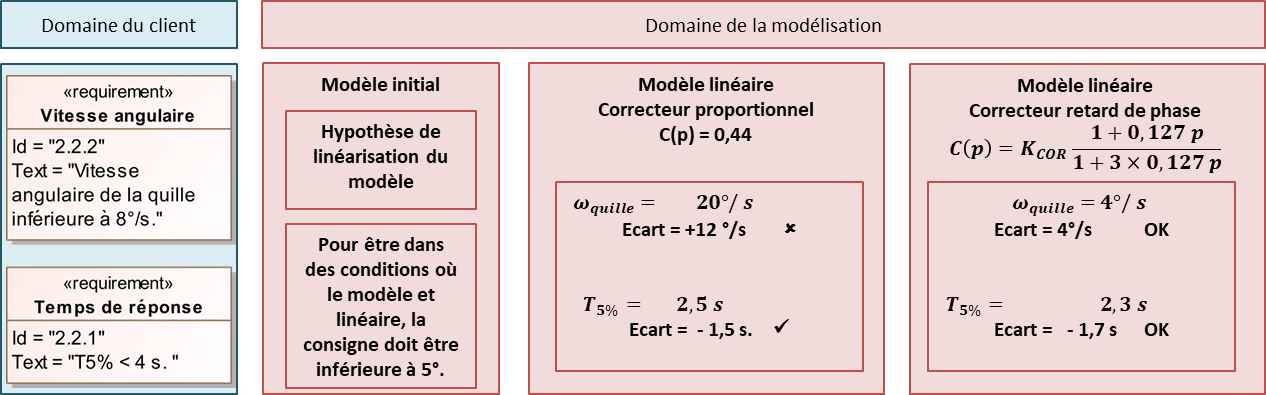
\includegraphics[width=\linewidth]{ecart_cor}
%\textit{}
\end{center}
\end{corrige}
\else
\fi

\ifprof
\else
\begin{marginfigure}
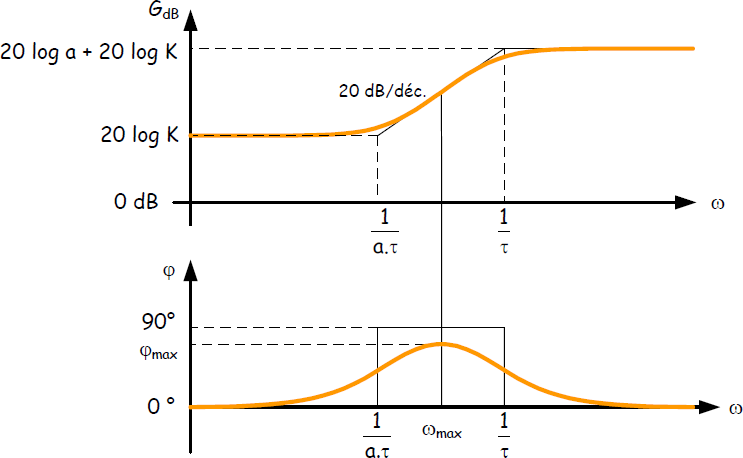
\includegraphics[width=\linewidth]{fig_09}
%\textit{}
\end{marginfigure}
\fi

\ifprof
\else
\begin{marginfigure}
\centering

\includegraphics[width=3cm]{Cy_03_01_Colle_RP_01_Quille_qr}
\end{marginfigure}
\fi

\ifprof
\else
\ifcolle
\else
\footnotesize
\marginnote{
\begin{solution}
\begin{enumerate}
\item $A_1=\dfrac{1}{Sp}$,  $A_2 = \dfrac{S2B}{V} $,  $A_3 = S$  et $A_4 = \dfrac{1}{Mp^2  +\lambda p  + k}$.
\item $H_1(p)=A_1  A_2A_3$ et $H_2 = \dfrac{A_4}{1+ A_2A_3A_4 }$.
\item $\dfrac{X(p)}{Q(p)}=\dfrac{2BS}{p\left(MVp^2  +\lambda pV  + kV+ 2BS^2\right) }$.
\item  $K_{\text{SV}} = \SI{2e-3}{m^3 s^{-1}V^{-1}}$. Pour $t<\SI{1,9}{s}$ : BO et  $t>\SI{1,9}{s}$ : BF.
\item 
\item $v(0^{+})=\SI{5,5}{V}$.
\item 
\item 
\item  $\omega_r \simeq \SI{4,5}{rad.s^{-1}}$.
\item $\Delta K = \SI{4,8}{dB}$.
\item 
\item $-10\log b$.
\item  $b=3,02$,  $T=\SI{0,127}{s}$,   $\phi\left(\omega^{*}\right) \simeq -28,79\degres $.
\item $t_5\%\simeq \SI{2,3}{s}<\SI{4}{s}$ $ 4 \degres/s< 8 \degres/s$.
\end{enumerate}
\end{solution}}
\normalsize
\fi
\fi
\ifprof
\else
\fi


\ifprof
\else


\begin{center}
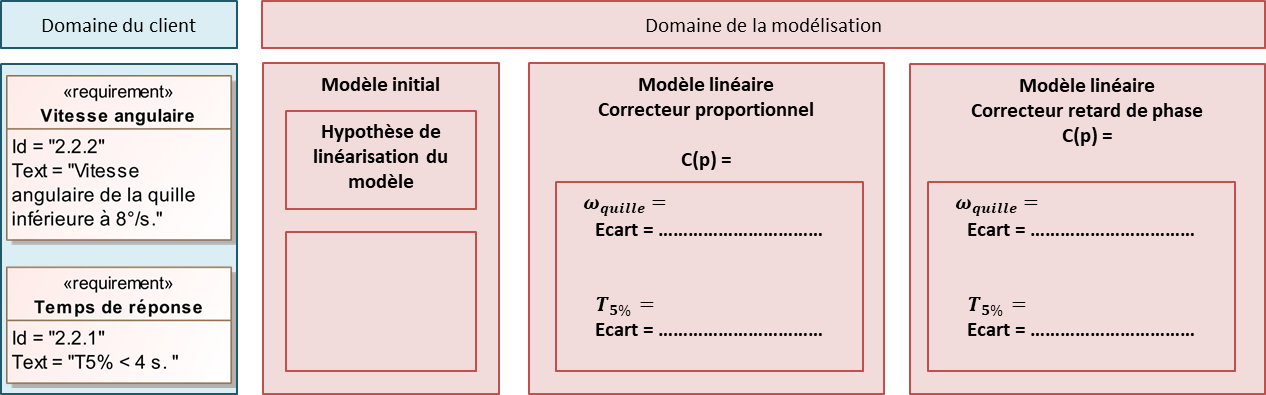
\includegraphics[width=\linewidth]{ecart}
%\textit{}
\end{center}

\begin{center}
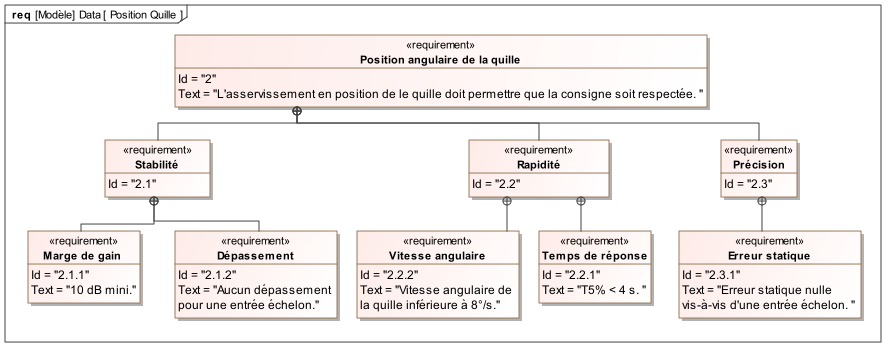
\includegraphics[width=.9\linewidth]{PositionQuille}
\end{center}


\fi
